\section{Estado documental e alcance da evidência}
\label{sec:estado}

A edição GEAR de outubro consolida o acervo em núcleo, adoção, guias, indicadores, exemplos, modelos, fundamentos e fontes. O \href{https://github.com/andrecodexvictor/GP-Pme/tree/8386586af110ba2112694a8ee6dd7b9d94d20572/framework}{núcleo documental versionado} permite inspecionar a especificação \citep{gppme2026repo}; o \href{https://github.com/andrecodexvictor/GP-Pme/tree/codex/gear-editorial/framework/publicacao}{registro de publicação} identifica o tratamento editorial e seus limites. Fontes externas, adaptações locais e exemplos ilustrativos têm funções distintas na argumentação.

A produção assistida e a auditoria são relatadas a partir desses documentos, da declaração de uso de IA e das correções registradas. A evidência permite examinar coerência e proveniência, mas não estabelecer a contribuição causal de cada ferramenta. Não há resultados de aplicação do GEAR em empresas, de prova de conceito no FrameSim ou de comparação com alternativas. Verificações de software do repositório não são usadas como validação do framework neste artigo.

\section{Protocolo prospectivo de prova de conceito}
\label{sec:protocolo}

\subsection{Perguntas e hipóteses de avaliação}

A prova de conceito futura no FrameSim será guiada por três perguntas. \textbf{PA1}: em empresas simuladas de 5 a 20 colaboradores, qual configuração produz planos mais completos e acionáveis para um conjunto comum de problemas? \textbf{PA2}: qual é o esforço humano e documental exigido para chegar a uma primeira decisão verificável? \textbf{PA3}: em quais condições de porte, maturidade, setor e comportamento das personas cada configuração falha ou exige adaptação?

A hipótese principal é que o GEAR oferece uma relação favorável entre cobertura e esforço nos cenários de baixa maturidade, sem pressupor que supere ITIL~4 ou COBIT~2019 em seus escopos de origem. Duas hipóteses secundárias serão examinadas: os mecanismos relacionais e a Fase Zero terão maior contribuição nos cenários com papéis acumulados; e a camada de IA reduzirá tempo de preparação somente quando contexto, revisão e critérios de saída forem mantidos. Nenhuma dessas hipóteses é tratada como confirmada nesta versão.

\subsection{Desenho pareado dos 25 casos}

Serão executados 25 blocos de teste, cada um correspondente a uma empresa sintética única. Em cada bloco, o mesmo manifesto de empresa, as mesmas personas, os mesmos eventos e o mesmo conjunto de tarefas serão submetidos a três configurações: GEAR, ITIL~4 adaptado e COBIT~2019 adaptado. Assim, 25 testes produzem 75 execuções de framework, mas a unidade de comparação permanece o caso pareado. Os IDs, setores, portes e desafios estão pré-especificados no \cref{ap:casos} e no arquivo suplementar \texttt{scenario-catalog.csv}.

Os casos serão estratificados em cinco faixas de porte (5--7, 8--10, 11--13, 14--16 e 17--20 colaboradores), com cinco empresas por faixa. Setores e incidentes variam para evitar que o resultado dependa de uma única narrativa. A maturidade inicial será limitada aos níveis 0, 1 e 2, coerentes com a porta de entrada do GEAR. Cada caso conterá ao menos uma tensão de direção, uma de fluxo de trabalho e uma de risco, mas sua severidade será balanceada antes das execuções.

\subsection{Configuração justa das alternativas}

A unidade avaliada não será o texto integral de cada referência, mas uma configuração declarada e reproduzível. O GEAR usará sua Fase Zero e seus três domínios essenciais. A configuração ITIL~4 usará princípios orientadores, cadeia de valor e um subconjunto documentado de práticas compatíveis com o pacote de tarefas. A configuração COBIT~2019 usará fatores de desenho e objetivos selecionados por critérios publicados antes do teste. Especialistas deverão revisar os dois baselines para evitar versões deliberadamente fracas.

Como ITIL e COBIT não possuem o mesmo escopo, os resultados serão divididos em dois painéis. O painel de \emph{desempenho no escopo comum} comparará somente tarefas que as três configurações se propõem a tratar. O painel de \emph{cobertura do problema completo} registrará lacunas em direção, serviço e segurança sem interpretar toda ausência como falha intrínseca do framework. Essa decomposição torna visível quando uma diferença decorre do escopo e quando decorre da execução.

No ensaio principal, qualquer assistência por LLM receberá o mesmo modelo, orçamento de contexto, temperatura, ferramentas e tempo entre os três braços. Agentes especializados exclusivos do GEAR não serão usados nessa comparação, pois confundiriam o efeito do conteúdo do framework com o efeito da implementação. A camada opcional de IA será examinada em uma ablação separada, GEAR manual versus GEAR assistido, depois do ensaio principal.

\subsection{Personas mais realistas e reprodutíveis}

Cada empresa terá um núcleo mínimo de quatro funções: proprietário ou direção, responsável por TI (interno ou terceirizado), dono de um processo de negócio e usuário afetado. Em empresas muito pequenas, uma pessoa poderá acumular funções, desde que o manifesto registre o conflito. As demais personas serão sorteadas de um catálogo compatível com setor e porte, sem introduzir cargos incompatíveis com uma equipe de até 20 pessoas.

Uma persona será descrita por cargo, poder decisório, tempo de empresa, disponibilidade semanal para governança, letramento digital, tolerância a risco, abertura à mudança, incentivos, objetivo, conflito, estilo de comunicação e até dois vieses cognitivos. Traços psicológicos não serão usados como diagnóstico clínico. Cada atributo deverá alterar uma regra observável da simulação; atributos puramente ornamentais serão removidos.

As personas do estudo serão sintéticas e não deverão representar indivíduos identificáveis. Antes do congelamento, o catálogo atualmente usado pelo FrameSim deverá passar por revisão de proveniência, licença e conteúdo; qualquer perfil derivado de pessoa real será removido ou transformado em arquétipo anônimo. Essa regra evita que o ganho de realismo seja obtido à custa de privacidade ou consentimento.

A aleatoriedade será hierárquica e registrada. A semente do caso define empresa e evento; a semente de equipe define a seleção e os traços das personas; e a semente de execução controla variações estocásticas. O mesmo manifesto congelado será reutilizado nos três braços. Amostragem aleatória simples será substituída por seleção restrita, verificando cobertura de papéis, soma de colaboradores, compatibilidade setorial, ausência de duplicatas e distribuição de resistência. Esse procedimento preserva diversidade sem perder comparabilidade.

\subsection{Pacote comum de tarefas}

Cada braço deverá responder ao mesmo pacote: (T1) diagnosticar a situação inicial e explicitar dados faltantes; (T2) priorizar cinco demandas concorrentes; (T3) tratar um incidente crítico sem apagar a fila normal; (T4) propor a linha de base de segurança e a evidência de restauração; (T5) transformar uma melhoria em entrega curta com responsável e critério de aceite; e (T6) produzir um painel de decisão com riscos, custos e próximos passos. O conjunto cobre direção, gestão de serviço, execução e segurança, permitindo também identificar lacunas de escopo.

\subsection{Métricas, rubrica e análise}

Os dois desfechos primários serão: \textbf{completude acionável}, pontuada de 0 a 100 por rubrica pré-publicada; e \textbf{esforço humano estimado}, em minutos para compreender, adaptar e aprovar a saída. A rubrica de completude verificará presença de responsável, prazo, entrada, saída, evidência, dependência e critério de encerramento. O esforço será estimado tarefa a tarefa por dois avaliadores e confrontado com número de rituais, papéis obrigatórios e artefatos produzidos.

Os desfechos secundários serão cobertura do pacote, rastreabilidade até fonte ou dado do caso, densidade documental, tempo computacional, custo de tokens, taxa de afirmações sem suporte por 100 afirmações verificáveis, número de correções HITL, violações de restrições, plausibilidade do cenário e aceitação simulada das personas. ``Aceitação simulada'' será reportada como comportamento do modelo, nunca como satisfação de trabalhadores reais.

Dois avaliadores humanos, cegos aos rótulos dos braços quando o conteúdo permitir, aplicarão a rubrica em ordem aleatória. Divergências serão resolvidas por consenso ou terceiro avaliador, e a concordância será reportada. O CriticAgent do FrameSim poderá apontar inconsistências, mas não será o juiz final. Falha do crítico, timeout ou resposta inválida produzirá valor ausente e log de erro; nunca uma nota substituta máxima.

Os resultados serão resumidos por mediana e intervalo interquartil. Diferenças pareadas por caso serão apresentadas com intervalos de confiança bootstrap. Se as premissas forem atendidas, o teste de Friedman examinará diferença global entre os três braços, seguido por comparações de Wilcoxon com correção de Holm e tamanho de efeito. Com 25 casos sintéticos, a análise terá caráter exploratório; valores de $p$ não serão usados para sugerir validade externa.

\begin{table}[htbp]
  \centering
  \caption{Tabela principal reservada para os resultados futuros. Traços indicam dados ainda não coletados.}
  \label{tab:resultados-planejados}
  \small
  \begin{tabular}{@{}lccc@{}}
    \toprule
    Métrica & GEAR & ITIL 4 adaptado & COBIT 2019 adaptado \\
    \midrule
    Completude acionável $\uparrow$ & -- & -- & -- \\
    Esforço humano (min) $\downarrow$ & -- & -- & -- \\
    Rastreabilidade (\%) $\uparrow$ & -- & -- & -- \\
    Afirmações sem suporte/100 $\downarrow$ & -- & -- & -- \\
    Correções HITL $\downarrow$ & -- & -- & -- \\
    \bottomrule
  \end{tabular}
\end{table}

\begin{figure}[H]
  \centering
  \IfFileExists{figures/generated/results-template.pdf}{%
    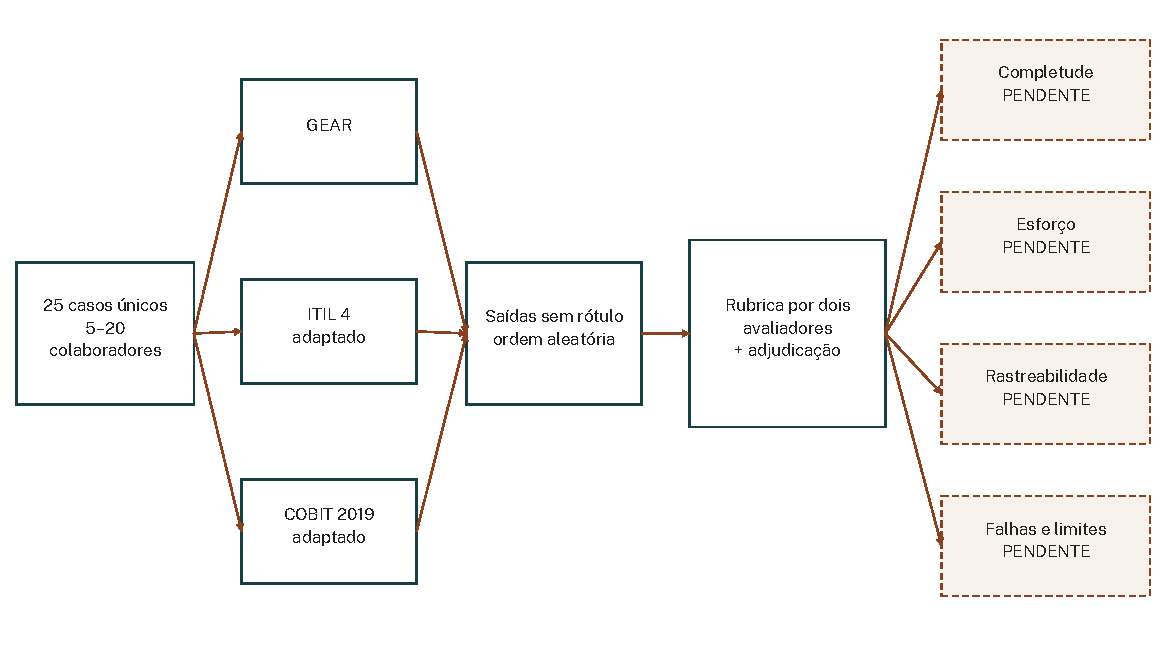
\includegraphics[width=0.95\textwidth]{figures/generated/results-template.pdf}%
  }{%
    \fbox{\parbox{0.88\textwidth}{\centering
      25 casos pareados $\rightarrow$ 3 configurações $\rightarrow$ rubrica cega $\rightarrow$ métricas e falhas $\rightarrow$ síntese comparativa (valores pendentes).}}
  }
  \caption{Modelo Mermaid para a síntese dos resultados. O diagrama representa o protocolo; não contém desempenho observado.}
  \label{fig:resultados-template}
\end{figure}

\subsection{Pré-condições no FrameSim}

O \href{https://github.com/andrecodexvictor/FrameSim}{FrameSim} é o ambiente previsto para a prova de conceito \citep{framesim2026repo}. Antes da coleta, sua versão deverá ser fixada e sua instrumentação conferida quanto a quatro requisitos: aleatoriedade semeada; reutilização de manifestos congelados entre os três braços; registro de erro ou dado ausente quando o avaliador automatizado falhar; e exportação de versões, parâmetros, prompts, fontes recuperadas e erros. São condições de aceitação do protocolo futuro, sem alegação de auditoria atual do código do simulador.

O atendimento e congelamento dessas condições deverá gerar um identificador de protocolo e um \emph{hash} para cada manifesto. Um teste piloto fora dos 25 casos verificará parsing, equilíbrio de tokens, cegamento dos rótulos e cálculo das métricas. O piloto poderá corrigir defeitos de instrumentação, mas não alterar hipóteses ou rubricas após a inspeção dos resultados principais.
